\justifying
\textbf{Цель работы:}
Определить диэлектрическую проницаемость слоя по данным рассеяния плоской электромагнитной волны.

\textbf{Задание:}
Пусть через горизонтальный слой диэлектрика из диспергирующей среды с электродинамическими параметрами $\varepsilon = \varepsilon_1(\omega) + i \varepsilon_2(\omega), \mu = 1 (\omega = 2 \pi f$ -- частота), распространяется плоская электромагнитная волна вдоль оси $Z$ снизу вверх. Пусть электрическая компонента поля направлена вдоль оси $Y$. Предполагается, что выше и ниже слоя находится вакуум. Пусть временной сигнал $E_{tr}(t, z)$ прошедшей волны в точке наблюдения с координатой $z > 0$ задан. Решить обратную задачу определения функции $\varepsilon(\omega)$. Для этого использовать итерационную последовательность Ньютона для восстановления коэффициента $n(\omega)$, а значит и $\varepsilon(\omega) = n ^ 2(\omega)$.

\textbf{Ход работы:}

Для начала выгрузим экспериментальные данные:
\begin{figure}[hb!]
    \centering
    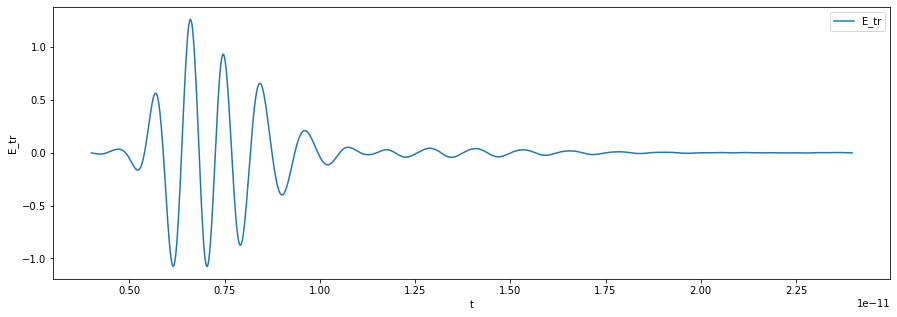
\includegraphics[width=\linewidth]{Figures/Experimental_data.png}
    \caption{Экспериментальные данные $E_{tr}(t)$}
    \label{fig:exp_data}
\end{figure}

Далее зададим спектр падающего электромагнитного импульса как гауссову функцию по формуле~(\ref{F_w}). Результат изображен на рисунке~(\ref{fig:F_w}).
\begin{equation}\label{F_w}
    F(\omega) = 2 \sqrt{\pi} \tau_{\pi} e ^ {-(\omega - \omega_0)^2 \tau_p^2}
\end{equation}

\begin{figure}[h!]
    \centering
    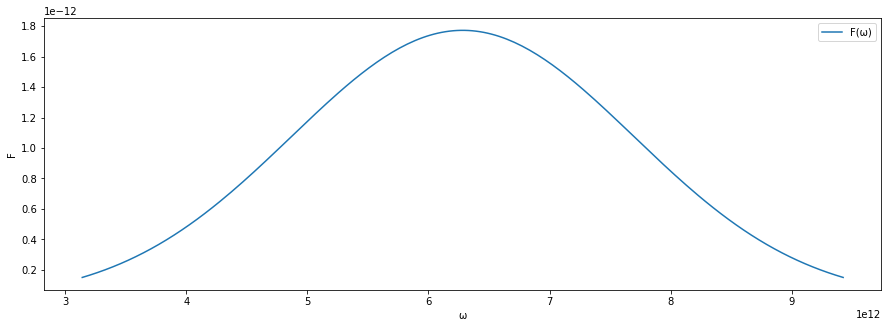
\includegraphics[width=\linewidth]{Figures/F_w.png}
    \caption{Cпектр падающего электромагнитного импульса $F(\omega)$}
    \label{fig:F_w}
\end{figure}

Коэффициент прохождения $T(\omega)$ вычисляется по формуле~(\ref{T_w}) и изображен на рисунке~(\ref{fig:T_w}).
\begin{equation}\label{T_w}
    T(\omega) = \frac{1}{F(\omega)} \int_{t_1}^{t_2} e^{i\omega(t-\frac{z}{c})} E_{tr}(t,z)dt
\end{equation}

Дальше используем итерационную последовательность Ньютона:
\begin{equation}
    n^{(m+1)} = n^{(m)} - \frac{\Phi(n^{(m)})}{\Phi'(n^{(m)})}
\end{equation}
для уравнения
\begin{equation}\label{F_w}
    \Phi(n) = \frac{4 n}{(n+1)^2e^{-ik_0nd} - (n-1)^2e^{ik_0nd}} - T(\omega) = 0
\end{equation}

После восстановления $n(\omega)$ можем получить $\varepsilon(\omega)$ по формуле:
\begin{equation}
    \varepsilon(\omega) = n^2(\omega)
\end{equation}


\begin{figure}[ht!]
    \centering
    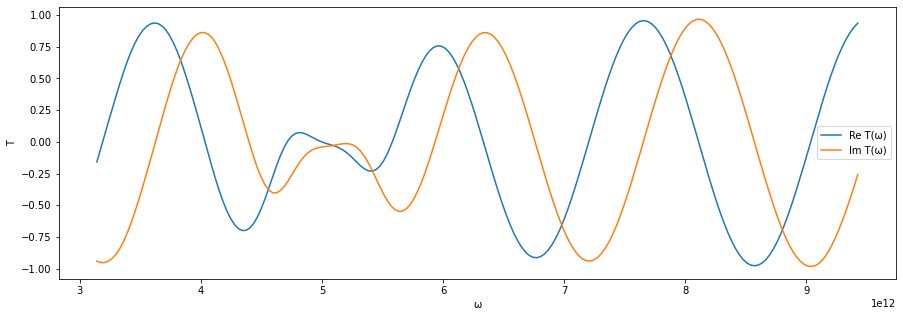
\includegraphics[width=\linewidth]{Figures/T_w.png}
    \caption{Коэффициент прохождения $T(\omega)$}
    \label{fig:T_w}
\end{figure}

Полученная диэлектрическая проницаемость $\varepsilon$ имеет реальную и мнимую части
\begin{equation}
    \varepsilon(\omega) = \varepsilon_1(\omega) + i\varepsilon_2(\omega),
\end{equation}
которые изображены на рисунке~(\ref{fig:epsilon}).

\begin{figure}[h!]
    \centering
    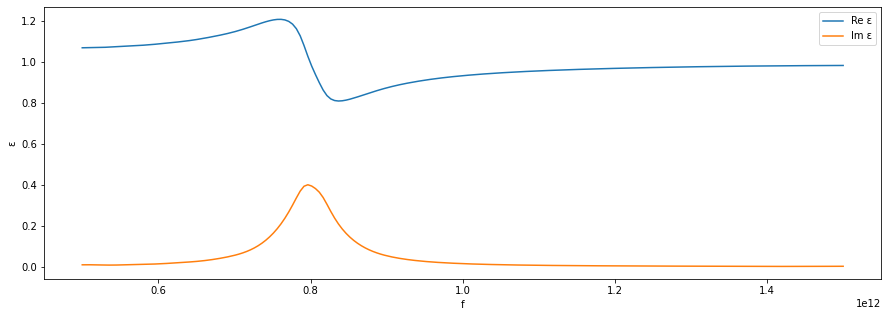
\includegraphics[width=\linewidth]{Figures/epsilon.png}
    \caption{Диэлектрическая проницаемость $\varepsilon$}
    \label{fig:epsilon}
\end{figure}
\newpage
\textbf{Выводы:}

В настоящей лабораторной работе была определена диэлектрическая проницаемость слоя по данным рассеяния плоской электромагнитной волны. Диспергирующая среда диэлектрического слоя обладала следующими электродинамическими параметрами: $\varepsilon = \varepsilon_1(\omega) + i \varepsilon_2(\omega), \mu = 1$. Предполагалось, что выше и ниже слоя находится вакуум. Временной сигнал $E_{tr}(t, z)$ наблюдался на фиксированном расстоянии $z = 10^{-3}$ м. При выполнении лабораторной работы была решена обратная задача определения функции $\varepsilon(\omega)$ с помощью итерационного метода Ньютона. Было получено, что пик диэлектрической проницаемости наблюдается при~$f~=~0.8$~ТГц.
